\documentclass[tikz,border=4mm]{standalone}
\usepackage[T1]{fontenc}
\usepackage{helvet}
\renewcommand{\familydefault}{\sfdefault}
\usetikzlibrary{arrows.meta,positioning,fit}

\begin{document}
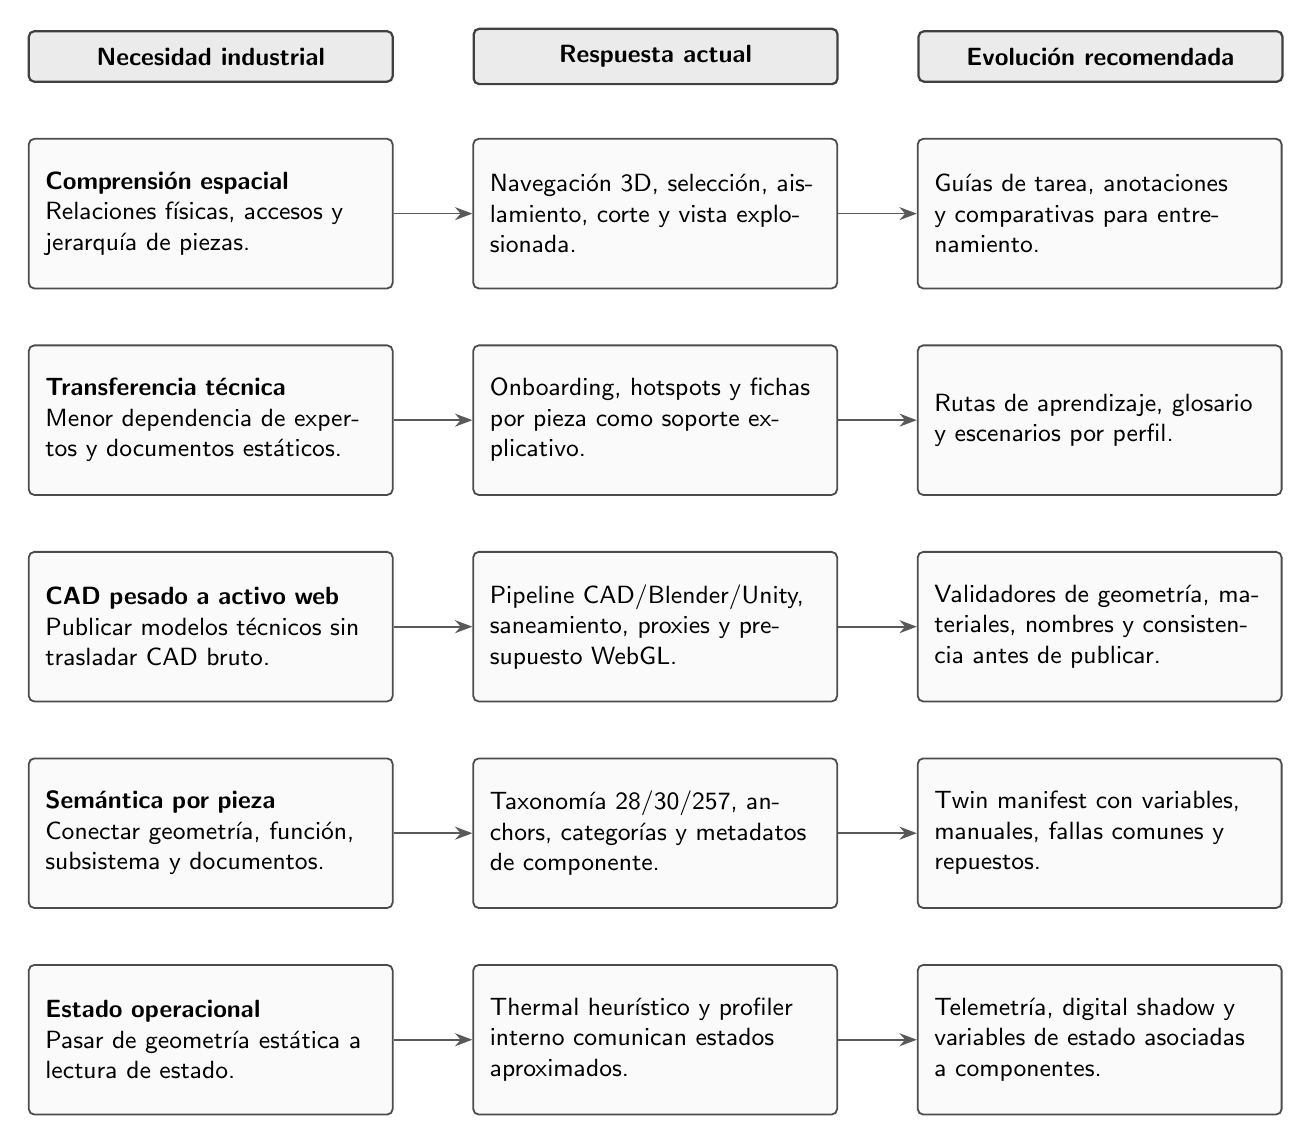
\begin{tikzpicture}[
  font=\sffamily\small,
  node distance=7mm and 10mm,
  header/.style={
    draw=black!75,
    rounded corners=2pt,
    line width=0.8pt,
    fill=black!8,
    align=center,
    inner sep=6pt,
    text width=42mm,
    font=\sffamily\bfseries\small
  },
  cell/.style={
    draw=black!70,
    rounded corners=2pt,
    line width=0.65pt,
    fill=black!2,
    align=left,
    inner sep=6pt,
    minimum height=19mm,
    text width=42mm
  },
  arrow/.style={-{Stealth[length=2.2mm]}, line width=0.6pt, draw=black!65}
]

\node[header] (h1) {Necesidad industrial};
\node[header, right=of h1] (h2) {Respuesta actual};
\node[header, right=of h2] (h3) {Evoluci\'on recomendada};

\node[cell, below=of h1] (n1) {\textbf{Comprensi\'on espacial}\\Relaciones f\'isicas, accesos y jerarqu\'ia de piezas.};
\node[cell, right=of n1] (r1) {Navegaci\'on 3D, selecci\'on, aislamiento, corte y vista explosionada.};
\node[cell, right=of r1] (e1) {Gu\'ias de tarea, anotaciones y comparativas para entrenamiento.};

\node[cell, below=of n1] (n2) {\textbf{Transferencia t\'ecnica}\\Menor dependencia de expertos y documentos est\'aticos.};
\node[cell, right=of n2] (r2) {Onboarding, hotspots y fichas por pieza como soporte explicativo.};
\node[cell, right=of r2] (e2) {Rutas de aprendizaje, glosario y escenarios por perfil.};

\node[cell, below=of n2] (n3) {\textbf{CAD pesado a activo web}\\Publicar modelos t\'ecnicos sin trasladar CAD bruto.};
\node[cell, right=of n3] (r3) {Pipeline CAD/Blender/Unity, saneamiento, proxies y presupuesto WebGL.};
\node[cell, right=of r3] (e3) {Validadores de geometr\'ia, materiales, nombres y consistencia antes de publicar.};

\node[cell, below=of n3] (n4) {\textbf{Sem\'antica por pieza}\\Conectar geometr\'ia, funci\'on, subsistema y documentos.};
\node[cell, right=of n4] (r4) {Taxonom\'ia 28/30/257, anchors, categor\'ias y metadatos de componente.};
\node[cell, right=of r4] (e4) {Twin manifest con variables, manuales, fallas comunes y repuestos.};

\node[cell, below=of n4] (n5) {\textbf{Estado operacional}\\Pasar de geometr\'ia est\'atica a lectura de estado.};
\node[cell, right=of n5] (r5) {Thermal heur\'istico y profiler interno comunican estados aproximados.};
\node[cell, right=of r5] (e5) {Telemetr\'ia, digital shadow y variables de estado asociadas a componentes.};

\foreach \a/\b in {n1/r1,r1/e1,n2/r2,r2/e2,n3/r3,r3/e3,n4/r4,r4/e4,n5/r5,r5/e5}
  \draw[arrow] (\a) -- (\b);

\end{tikzpicture}
\end{document}
